\documentclass[../../main.tex]{subfiles}
\begin{document}
\section{Definition und Beispiele von Vektorräumen, Untervektorräume}

\begin{df}\mbox{}\label{6.1.1}
[$\to$ \ref{3.1.1}] Ein \emph{Vektorraum}\index{Vektorraum@{\bf Vektorraum}} (\emph{VR}) ist ein Tupel $(K,+_K,\cdot_K, V,+,\cdot)$, wobei $(K,+_K,\cdot_K)$ ein Körper, $(V,+)$ eine abelsche Gruppe [$\to$ \ref{2.1.1}] und $\cdot:K\times V\to V$ eine (meist unsichtbar oder infix geschriebene) Abbildung ist mit folgenden Eigenschaften:
\begin{itemize}
\item[(V)] $\forall a,b\in K:\forall v\in V:(a\cdot_K b)v = a(bv)$ \qquad"`verträglich"'
\item[\vecN] $\forall v\in V: 1_Kv = v$\index{neutrales Element@{\bf neutrales Element}}
\item[\vecD] $\forall a\in K: \forall v,w\in V: a(v+w) = (av)+(aw)$\index{distributiv@{\bf distributiv}}
\item[(D')] $\forall a,b\in K:\forall v\in V: (a+_Kb)v = (av) + (bv)$\index{distributiv@{\bf distributiv}}
\end{itemize}
\end{df}

\begin{bem}\label{6.1.2}
Sei $(K,+_K,\cdot_K,V,+,\cdot)$ ein Vektorraum.
\begin{enumerate}[\normalfont(a)]
\item Die Elemente von $V$ nennt man oft \emph{Vektoren}\index{Vektorraum@{\bf Vektorraum}!Vektoren}. Wir bezeichnen sie oft mit\\
$v,w,u,x,y,\dots$. Früher bezeichnete man sie mit $\overrightarrow v, \overrightarrow w,\dots$
\item Die Elemente von $K$ nennt man oft \emph{Skalare}\index{Vektorraum@{\bf Vektorraum}!Skalare}. Wir bezeichnen sie oft mit $a,b,c,d,\lambda,\mu,$\\
$\alpha,\beta, \gamma, \delta,\ldots$
\item Sprechweisen:
\begin{itemize}
\item $(K,+_K,\cdot_K)$ Grund-/Skalarkörper\index{Vektorraum@{\bf Vektorraum}!Grundkörper}
\item $V$ zugrundeliegende (oder Träger-)Menge\index{Vektorraum@{\bf Vektorraum}!Trägermenge}
\item $(V,+)$ zugrundeliegende abelsche Gruppe oder additive Gruppe.\index{Vektorraum@{\bf Vektorraum}!additive Gruppe}
\item $+$ (Vektor-)Addition\index{Vektorraum@{\bf Vektorraum}!Vektoraddition}
\item $\cdot$ Skalarmultiplikation (nicht verwechseln mit Skalarprodukt!)\index{Vektorraum@{\bf Vektorraum}!Skalarmultiplikation}
\end{itemize}
\item "`Punkt vor Strich"' [$\to$ \ref{3.1.2} (f)]: $av+bw = (av)+(bw)$ für $a,b\in K, v,w\in V$.
\item \vecD~ besagt, dass für jedes $a\in K$ die Abbildung $V\to V, v\mapsto av$ ein Gruppenendomorphismus von $(V,+)$ ist. Insbesondere $a\cdot 0=0$ und $a(-v) = -av$ für alle $a\in K$ [$\to$ \ref{3.1.2} (g)].
\item Für alle $v\in V$ gilt $0_K \cdot v = 0$, denn $0_Kv+0_Kv \overset{\text{(D')}}{=} (0_K+_K0_K) v \overset{\text{(N)}}{=}0_K v$.
\item Für alle $a\in K$ gilt $(-a)v = -av$, denn $av + (-a)v \overset{\text{(D')}}{=} (a-_Ka)v = 0_K v \overset{\text{(f)}}{=} 0$.
\end{enumerate}
\end{bem}

\begin{sprnt}\mbox{}\label{6.1.3}
[$\to$ \ref{2.1.2} (e), \ref{3.1.2} (d)] Statt von einem Vektorraum $(K, +_K,\cdot_K, V,+,\cdot)$ spricht man auch von einem $K$-Vektorraum $V$ oder von einem Vektorraum $V$ (über $K$). Statt $+_K$ und $\cdot_K$ schreibt man $+$ und $\cdot$.
\end{sprnt}

\begin{bsp}\label{6.1.4}
\begin{enumerate}[\normalfont(a)]
\item Jede einelementige abelsche Gruppe $V=\left\{0\right\}$ kann man für jeden Körper $K$ auf genau eine Weise zu einem $K$-Vektorraum machen (nämlich indem man die Skalarmultiplikation durch $\lambda\cdot 0 := 0$ für $\lambda \in K$ definiert). Man nennt dann $V$ einen \emph{Nullvektorraum}.
\item Sei der Körper $K$ ein Unterring [$\to$ \ref{3.2.1}] des kommutativen Ringes $A$ [$\to$ \ref{3.1.1}]. Dann ist $A$ ein $K$-Vektorraum vermöge der Skalarmultiplikation $\cdot:K\times A\to A, (\lambda, a) \mapsto \lambda\cdot_A a$.

Zum Beispiel wird in dieser Weise der Polynomring $K[X]$ ein $K$-Vektorraum und die komplexen Zahlen bilden einen reellen Vektorraum (d.h. $\C$ ist ein $\R$-Vektorraum). Es ist $\C$ aber auch ein $\C$-Vektorraum. Allgemeiner ist jeder Körper ein Vektorraum über sich selbst, das heißt $K$ ist ein $K$-Vektorraum vermöge der Körpermultiplikation als Skalarmultiplikation.
\item Ist $A$ eine Menge, so wird die abelsche Gruppe $\Pow(A)$ aus \ref{2.1.3} (e) ein $\F_2$-Vektorraum vermöge
$$0_{\F_2}B := \emptyset \text{ und } 1_{\F_2}B := B \text{ für } B\in \Pow(A).$$
\end{enumerate}
\end{bsp}

\begin{satdef}\label{6.1.5}
{\rm[$\to$ \ref{2.1.11}]} Sei $K$ ein Körper, $I$ eine Menge und für jedes $i\in I$ ein $K$-Vektorraum $V_i$ gegeben. Das in \ref{2.1.11} definierte direkte Produkt $\prod_{i\in I}V_i$ der additiven Gruppe der $V_i$ wird dann vermöge der "`punktweisen"' Skalarmultiplikation
$$K\times \prod_{i\in I}V_i\to \prod_{i\in I}V_i, (a,f)\mapsto (i\mapsto af(i))$$
zu einem $K$-Vektorraum, dem \emph{direkten Produkt}\index{Vektorraum@{\bf Vektorraum}!direktes Produkt} der $K$-Vektorräume $V_i$ $(i\in I)$. Für $a\in K$ und $f\in \prod_{i\in I}V_i$ gilt $(af)(i) = a f(i)$ für alle $i\in I$.
\end{satdef}
\begin{proof}
Übung.
\end{proof}

\begin{kor}\label{6.1.6}
{\rm[$\to$ \ref{2.1.12}]} Sei $K$ ein Körper. Sind $n\in \N_0$ und $V_1,\ldots,V_n$ $K$-Vektorräume, so ist die abelsche Gruppe $V_1\times \ldots\times V_n$ zusammen mit der durch
$$a\cvec{v_1\\\vdots\\v_n} := \cvec{av_1\\\vdots\\av_n} ~(a\in K, v_1\in V_1, \ldots, v_n\in V_n)$$
definierte Skalarmultiplikation ein $K$-Vektorraum (wir schreiben hier $n$-Tupel wieder als "`Spaltenvektoren"'). Insbesondere wird auf diese Weise für jeden $K$-Vektorraum $V$ und jedes $n\in\N_0$ die abelsche Gruppe $V^n = \underbrace{V\times \ldots\times V}_{n\text{-mal}}$ ein $K$-Vektorraum.
\end{kor}

\begin{bem}\label{6.1.7}
Sei $K$ ein Körper und $n\in \N_0$. Als sehr wichtiger Spezialfall von \ref{6.1.6} ergibt sich $K^n$ ist mit der durch
$$\lambda\cvec{a_1\\\vdots\\a_n}:=\cvec{\lambda a_1\\\vdots\\\lambda a_n}\qquad(\lambda\in K, a_1,\ldots,a_n\in K)$$
[$\to$\text{\ref{5.1.3}(c)}] definierten Skalarmultiplikation ein $K$-Vektorraum (beachte $K^0=\left\{()\right\}=\{0\}$ ist ein Nullvektorraum [$\to$ \ref{6.1.4} (a)]).
\end{bem}

\begin{bsp}\label{6.1.8}
$\R^n=\underbrace{\R\times \ldots\times \R}_{n-\text{mal}}$
\begin{center}
\begin{tikzpicture}
\draw[->, thick] (-2.5,0) -- (3,0) node[anchor = south]{$\R$};
\draw[->, thick] (0,-1.5) -- (0,3.5) node[anchor = east]{$\R$};

\node(0){};
\node[above right = 5 of 0]{$\R^2$};
\node[below right = 2 of 0]{$\cvec{a_1\\a_2}+\cvec{b_1\\b_2}=\cvec{a_1+b_1\\a_2+b_2}$};
\node[above left = 3 of 0]{$2\cvec{c_1\\c_2} = \cvec{2c_1\\2c_2}$};
\draw (1, 2pt) -- (1, -2pt) node[anchor = north]{$a_1$};
\draw (1.5, 2pt) -- (1.5, -2pt) node[anchor = north]{$b_1$};
\draw (2pt, .5) -- (-2pt, .5) node[anchor = east]{$a_2$};
\draw (2pt, 2.5) -- (-2pt, 2.5) node[anchor = east]{$b_2$};
\draw (2.5, 2pt) -- (2.5, -2pt) node[anchor = north]{$a_1+b_1$};
\draw (2pt , 3) -- (-2pt, 3) node[anchor = east]{$a_2+b_2$};
\draw (-1, 2pt) -- (-1, -2pt) node[anchor = south]{$c_1$};
\draw (2pt, -.5) -- (-2pt, -.5) node[anchor = west]{$c_2$};
\draw (-2, 2pt) -- (-2, -2pt) node[anchor = south]{$2c_1$};
\draw (2pt, -1) -- (-2pt, -1) node[anchor = west]{$2c_2$};

\draw[->, blue] (0,0) -- (1,.5);
\draw[green,densely dashed] (1,0) -- (1,.5);
\draw[green,densely dashed] (0,0.5) -- (1,.5);
\draw[->, red] (0,0) -- (1.5,2.5);
\draw[green,densely dashed] (1.5,0) -- (1.5,2.5);
\draw[green,densely dashed] (0,2.5) -- (1.5,2.5);
\draw[->, blue] (1.5,2.5) -- (2.5,3);
\draw[green,densely dashed] (2.5,0) -- (2.5,3);
\draw[green,densely dashed] (0,3) -- (2.5,3);
\draw[->, red] (1,.5) -- (2.5,3);
\draw[->] (0,0) -- (-1, -.5);
\draw[green,densely dashed] (-1,0) -- (-1, -.5);
\draw[green,densely dashed] (0,-0.5) -- (-1, -.5);
\draw[dashed, ->] (-1,-.5) -- (-2,-1);
\draw[green,densely dashed] (-2,0) -- (-2,-1);
\draw[green,densely dashed] (0,-1) -- (-2,-1);
\end{tikzpicture}
\end{center}
Vektoraddition: Aneinanderfügen von Pfeilen\\
Skalarmultiplikation: Strecken
\end{bsp}

\red{Bis hierher sollten wir am 9. Dezember kommen.}

\begin{df}\mbox{}\label{6.1.9}
[$\to$ \ref{2.2.1}, \ref{3.2.1}] Seien $U$ und $V$ $K$-Vektorräume. Dann heißt $U$ ein \emph{Untervektorraum} oder \emph{(linearer) Unterraum}\index{Vektorraum@{\bf Vektorraum}!Untervektorraum/linearer Unterraum} (\emph{UR}) von $V$, wenn die additive Gruppe [$\to$~\ref{6.1.2}] von $U$ eine Untergruppe der additiven Gruppe von $V$ ist und
\[\forall a\in K:\forall u\in U: a\cdot_U u = a\cdot_V u.\]
\end{df}

\begin{pro}\label{6.1.10}
{\rm[$\to$ \ref{2.2.2}, \ref{3.2.2}]} Sei $V$ ein $K$-Vektorraum und $U$ eine Menge. Dann ist $U$ genau dann Trägermenge eines Unterraums von $V$, wenn gilt:
\begin{enumerate}[\rm(a)]
\item $U\subseteq V$,
\item $0_V\in U$,
\item $\forall u,v\in U: u +_V v \in U$ und
\item $\forall \lambda\in K:\forall u\in U:\lambda \cdot_V u \in U$.
\end{enumerate}
In diesem Fall gibt es \emph{genau} ein Paar $(+_U,\cdot_U)$, mit dem $(K,+_K,\cdot_K,U,+_U,\cdot_U)$ ein Unterraum von $(K,+_K,\cdot_K, V, +_V,\cdot_V)$ wird. Es gilt dann
\begin{enumerate}[\rm(a')]
\item $0_U = 0_V$,
\item $\forall u,v\in U:u+_U v = u+_V v$ und
\item $\forall \lambda\in K:\forall u\in U:\lambda\cdot_Uu= \lambda\cdot_Vu$.
\end{enumerate}
\end{pro}
\begin{proof}
Einfach mit \ref{2.2.2} unter Verwendung von $-_V u\overset{\text{\ref{6.1.2} (g)}}{=} (-1)\cdot_V u$ für alle $u\in V$.
\end{proof}

\begin{bsp}\label{6.1.11}
\begin{enumerate}[\normalfont(a)]
\item Ist $K$ ein Körper, so ist die Lösungsmenge eines \emph{homogenen} linearen Gleichungssystems über $K$ [$\to$ \ref{5.1.1}] in $n$ Unbekannten ein Untervektorraum des Vektorraums $K^n$. Dies besagt gerade \ref{5.1.3}.
\item Die Mengen $\R$ der reellen und $\left\{a\i\mid a\in\R\right\}$ der \emph{rein imaginären} Zahlen sind jeweils Unterräume des $\R$-Vektorraums $\C$, aber nicht des $\C$-Vektorraums $\C$.
\item Ist $K$ ein Körper, so ist für jedes $d\in\left\{-\infty\right\}\cup \N_0$
\[K[X]_d := \left\{p\in K[X]\mid\deg p\le d\right\}\]
ein Unterraum des $K$-Vektorraums $K[X]$ (unsauber gesagt: ein $K$-Unterraum von $K[X]$).
\end{enumerate}
\end{bsp}

\begin{pro}\label{6.1.12}
{\rm[$\to$ \ref{2.2.5}, \ref{3.3.8}]} Sei $V$ ein $K$-Vektorraum und $M$ eine Menge von Unterräumen von $V$. Dann ist $\bigcap M$ ein Unterraum von $V$ (mit $\bigcap \emptyset := V$).
\end{pro}
\begin{proof}
Einfach mit \ref{2.2.5}.
\end{proof}

\begin{satdef}\label{6.1.13}
{\rm[$\to$ \ref{2.2.6}, \ref{3.3.9}]} Sei $V$ ein $K$-Vektorraum und $E\subseteq V$. Dann gibt es \emph{\underline{\underline{den}} kleinsten}\index{Vektorraum@{\bf Vektorraum}!Unterraum!erzeugter Unterraum/ lineare Hülle/ Spann} Unterraum $U$ von $V$ mit $E\subseteq U$. Man nennt ihn den von $E$ in $V$ \case{\emph{erzeugten}}{\emph{aufgespannten}} Unterraum oder \case{die lineare Hülle}{den Spann} von $E$ (in $V$) und notiert in mit $\spann{E}$.
\end{satdef}
\begin{proof}
Völlig analog zum Beweis von \ref{2.2.6} (benutze \ref{6.1.12} statt \ref{2.2.5}).
\end{proof}

\begin{sat}\label{6.1.14}
{\rm[$\to$ \ref{2.2.7}, \ref{3.3.10}]} Sei $V$ ein $K$-Vektorraum und $E\subseteq V$. Dann
$$\spann{E} = \Bigg\{\underbrace{\sum_{i=1}^{n}\lambda_i v_i}_\text{"`Linearkombinationen"'}\Bigg|~ n\in \N_0, \lambda_1,\ldots,\lambda_n\in K, v_1,\ldots,v_n\in E\Bigg\}.$$
\end{sat}
\begin{proof}
Der Beweis ist analog zum Beweis von Satz \ref{2.2.7} und stellt gleichzeitig einen neuen Beweis für \ref{6.1.13} dar.
\end{proof}

\section{Basen}

\begin{df}\label{6.2.1}
Seien $V$ ein $K$-Vektorraum, $n\in\N_0$ und $v_1,\dots,v_n\in V$.
\begin{enumerate}[\normalfont(a)]
\item Man nennt
$$\lin(v_1,\dots,v_n):=\lin(\{v_1,\dots,v_n\})\overset{\text{\ref{6.1.1}(D')}}=\Set{\sum_{i=1}^n\la_iv_i|\la_1,\dots,\la_n\in K}$$
den Spann von $v_1,\dots,v_n$ [$\to$\ref{5.1.5}, \ref{6.1.13}, \ref{6.1.14}].
Man sagt, $v_1,\dots,v_n$ \emph{erzeugen}\index{Vektorraum@{\bf Vektorraum}!Erzeugendensystem} $V$ (oder \emph{spannen} $V$ auf oder bilden ein \emph{Erzeugendensystem} von $V$), wenn $$V=\lin(v_1,\dots,v_n).$$
\item Man nennt $v_1,\dots,v_n$ \emph{linear unabhängig}\index{Vektorraum@{\bf Vektorraum}!lineare Unabhängigkeit}, wenn
$$\lin(v_1,\dots,v_{i-1},v_{i+1},\dots,v_n)\ne\lin(v_1,\dots,v_n)$$
für alle $i\in\{1,\dots,n\}$. Andernfalls nennt man $v_1,\dots,v_n$ \emph{linear abhängig}
\item Es heißt $(v_1,\dots,v_n)$ eine \emph{(geordnete) Basis}\index{Vektorraum@{\bf Vektorraum}!Basis} von $V$, falls $v_1,\dots,v_n$ linear unabhängig sind und $V$ erzeugen. Man sagt dann auch, $v_1,\dots,v_n$
\emph{bilden} eine Basis von $V$.
\end{enumerate}
\end{df}

\begin{bsp}\label{6.2.2}
Sei $K$ ein Körper und $n\in\N_0$. Ist für $i\in\{1,\dots,n\}$
$$e_i:=\left(\begin{smallmatrix}0\\\vdots\\0\\1\rlap{\tiny $\longleftarrow$ $i$-te Stelle}\\0\\\vdots\\0\end{smallmatrix}\right)\qquad\qquad\in K^n$$
der $i$-te \emph{Standardvektor} (oder \emph{kanonische Einheitsvektor}) im $K^n$, so ist
$$\underline e:=(e_1,\dots,e_n)$$
eine Basis des $K^n$. Man nennt sie die \emph{Standardbasis}\index{Vektorraum@{\bf Vektorraum}!Basis!Standardbasis} (auch natürliche Basis oder kanonische Basis) des $K^n$.
\end{bsp}

\begin{pro}\label{6.2.3}
Seien $V$ ein $K$-Vektorraum, $n\in\N_0$ und $v_1,\dots,v_n\in V$. Dann sind folgende Aussagen äquivalent:
\begin{enumerate}[\rm(a)]
\item $v_1,\dots,v_n$ sind linear unabhängig.
\item $\forall\la_1,\dots,\la_n\in K:(\la_1v_1+\ldots+\la_nv_n=0\implies \la_1=\ldots=\la_n=0)$, das heißt "`der Nullvektor lässt sich aus den $v_i$ nur trivial kombinieren"'.
\end{enumerate}
\end{pro}

\begin{proof}
Die logischen Negationen von (a) und (b) sind:
\begin{enumerate}[\normalfont(a)]
\item[(\=a)] Es gibt ein $i\in\{1,\dots,n\}$ mit $\lin(v_1,\dots,v_{i-1},v_{i+1},\dots,v_n)=\lin(v_1,\dots,v_n)$.
\item[(\=b)] Es gibt $i\in\{1,\dots,n\}$ und $\la_1,\dots,\la_n\in K$ mit $\la_1v_1+\dots+\la_nv_n=0$ und $\la_i\ne0$.
\end{enumerate}
Wir zeigen, dass für alle $i\in\{1,\dots,n\}$ äquivalent sind:
\begin{enumerate}[\normalfont(a)]
\item[(\~a)] $\lin(v_1,\dots,v_{i-1},v_{i+1},\dots,v_n)=\lin(v_1,\dots,v_n)$.
\item[(\~b)] Es gibt $\la_1,\dots,\la_n\in K$ mit $\la_1v_1+\dots+\la_nv_n=0$ und $\la_i\ne0$.
\end{enumerate}
Dies ist klar, da (\~a) und (\~b) beide äquivalent sind zu $v_i\in\lin(v_1,\dots,v_{i-1},v_{i+1},\dots,v_n)$.
\end{proof}

\begin{bem}\label{6.2.4}
\begin{enumerate}[\normalfont(a)]
\item In §\ref{5.1} hatten wir gesehen, wie man aus einer gegebenen Matrix in reduzierter Stufenform eine Basis ihres Kerns ablesen kann [$\to$\ref{5.1.14}(a)].
\item Die Nichtnullzeilen einer Matrix in Stufenform [$\to$\ref{5.1.10}] bilden eine Basis ihres Zeilenraums. In der Tat: Sie spannen den Zeilenraum gemäß seiner Definition \ref{5.3.1} natürlich auf. Um zu zeigen, dass sie linear unabhängig sind, bezeichne $r$ die Anzahl der Stufen und $a^{(i)}$ die $i$-te Zeile für jedes $i\in\{1,\dots,r\}$. Seien
$\la_1,\dots,\la_r\in K$ mit $\sum_{i=1}^r\la_ia^{(i)}=0$. Angenommen es gilt nicht $\la_1=\dots=\la_r=0$. Dann gibt es ein $k\in\{1,\dots,r\}$ mit
$\la_1=\dots=\la_{k-1}=0\ne\la_k$. Ist $j_k$ die $k$-te Stufenposition der Matrix, so folgt nun $\la_ka^{(k)}_{j_k}=0$ und daher $\la_k=0$. Widerspruch!
$$\begin{pmatrix}
\tikz[baseline=(s1.base)]\node(s1){1}; & \tikz[baseline=(se.base)]\node(se){7}; &   &   & \tikz\node(r1){};\\
\tikz[baseline=(n1.base)]\node(n1){0}; & \tikz[baseline=(s2.base)]\node(s2){3}; &   &   & \tikz\node(r2){};\\
\tikz\node(l3){};  & \tikz[baseline=(n2.base)]\node(n2){0}; & \tikz[baseline=(s3.base)]\node(s3){4}; &   & \tikz\node(r3){};\\
\tikz\node(l4){};  &   & \tikz[baseline=(n3.base)]\node(n3){0}; & \tikz[baseline=(s4.base)]\node(s4){1}; & \tikz\node(r4){};\\
\tikz\node(l5){};  &   &   & \tikz[baseline=(n4.base)]\node(n4){0}; & \tikz[baseline=(s5.base)]\node(s5){2}; \\
 &   &   &   & \tikz[baseline=(n5.base)]\node(n5){0}; \\
  ~\\
\tikz[baseline=(n6.base)]\node(n6){0}; & \tikz[baseline=(n7.base)]\node(n7){0}; & \tikz[baseline=(n8.base)]\node(n8){0}; & \tikz[baseline=(n9.base)]\node(n9){0}; & \tikz[baseline=(n10.base)]\node(n10){0};
\end{pmatrix} 
\begin{array}{cl}
(1):& 1\la_1 = 0\\
(2):& \underbrace{7\la_1}_{=0} + 3\la_2 = 0\\
\vdots
\end{array}
\begin{tikzpicture}[overlay]
\draw (s1.north west) -- (s1.south west) -- (s2.north west) -- (s2.south west) -- (s3.north west) -- (s3.south west) -- (s4.north west) -- (s4.south west) -- (s5.north west) -- (s5.south west) -- (s5.south east);
\draw[loosely dotted, very thick] (n1) -- (n6);
\draw[loosely dotted, very thick] (n2) -- (n7);
\draw[loosely dotted, very thick] (n3) -- (n8);
\draw[loosely dotted, very thick] (n4) -- (n9);
\draw[loosely dotted, very thick] (n5) -- (n10);

\draw[opacity=.2,line width=5 mm,line cap=round,color=red] (s1.west) to (r1.east);
\draw[opacity=.2,line width=5 mm,line cap=round,color=red] (n1.west) to (r2.east);
\draw[opacity=.2,line width=5 mm,line cap=round,color=red] (l3.west) to (r3.east);
\draw[opacity=.2,line width=5 mm,line cap=round,color=red] (l4.west) to (r4.east);
\draw[opacity=.2,line width=5 mm,line cap=round,color=red] (l5.west) to (s5.east);

\node[left = 0.2 of s1]{$a^{(1)}$};
\node[left = 0.2 of n1]{$a^{(2)}$};
\node[left = 0.2 of l3]{$a^{(3)}$};
\node[left = 0.2 of l4]{$a^{(4)}$};
\node[left = 0.2 of l5]{$a^{(5)}$};

\draw[opacity=.2,line width=5 mm,line cap=round,color=blue] (s1.north) to (n6.south);
\node[below = 0 of n6]{(1)};
\draw[opacity=.2,line width=5 mm,line cap=round,color=blue] (se.north) to (n7.south);
\node[below = 0 of n7]{(2)};
\node[below = 0 of n8]{\dots};
\end{tikzpicture}$$
\item Bemerkungen (a) und (b) zeigen, wie man mit dem Gauß-Verfahren aus §\ref{5.2} zu einer gegebenen Matrix $A\in K^{m\times n}$ ($K$ ein Körper) Basen der
Untervektorräume $\ker A$ und $\row A$ des $K$-Vektorraums $K^n$ berechnen kann.
\end{enumerate}
\end{bem}


\begin{lem}[Austauschlemma von Steinitz]{\rm[\href{http://de.wikipedia.org/wiki/Ernst_Steinitz}{Ernst Steinitz} *1871 \dag 1928]}\label{6.2.5}\\
Sei $(v_1,\dots,v_n)$ eine Basis des $K$-Vektorraums $V$. Seien $\la_1,\dots,\la_n\in K$, $w=\sum_{i=1}^n\la_iv_i$ und $j\in\{1,\dots,n\}$ mit $\la_j\ne0$. Dann ist auch
$(v_1,\dots,v_{j-1},w,v_{j+1},\dots,v_n)$ eine Basis von $V$.
\end{lem}
\begin{proof}
Wegen $$v_j=\frac1{\la_j}\left(\sum_{\over{i=1}{i\ne j}}^n(-\la_i)v_i+1w\right)$$
gilt $v_i\in\lin(v_1,\dots,v_{j-1},w,v_{j+1},\dots,v_n)$ für alle $i\in\{1,\dots,n\}$ und daher
$$\lin(v_1,\dots,v_{j-1},w,v_{j+1},\dots,v_n)=V.$$ Es ist noch zu zeigen, dass $v_1,\dots,v_{j-1},w,v_{j+1},\dots,v_n$ linear unabhängig sind. Seien hierzu
$\mu_1,\dots,\mu_n\in K$ mit
$$\sum_{\over{i=1}{i\ne j}}^n\mu_iv_i+\mu_jw=0.$$ Zu zeigen ist $\mu_i=0$ für alle $i\in\{1,\dots,n\}$. Es gilt
$$0=\sum_{\over{i=1}{i\ne j}}^n\mu_iv_i+\mu_j\sum_{\over{i=1}{i\ne j}}^n\la_iv_i+\mu_j\la_jv_j=
\sum_{\over{i=1}{i\ne j}}^n(\mu_i+\mu_j\la_i)v_i+\mu_j\la_jv_j.$$
Da $v_1,\dots,v_n$ linear unabhängig sind, folgt $\mu_j=0$ (denn $\mu_j\la_j=0$ und $\la_j\ne0$) und somit
$\mu_i=\mu_i+\mu_j\la_i=0$ für alle $i\in\{1,\dots,n\}\setminus\{j\}$.
\end{proof}

\begin{sat}[Austauschsatz von Steinitz]\label{6.2.6}
Sei $(v_1,\dots,v_n)$ eine Basis des Vektorraums $V$ und seien $w_1,\dots,w_m\in V$ linear unabhängig. Dann gibt es paarweise verschiedene
$i_1,\dots,i_m\in\{1,\dots,n\}$ so, dass $v_1,\dots,v_n$ nach Ersetzen von $v_{i_j}$ durch $w_j$ {\rm($j\in\{1,\dots,m\}$)} immer noch eine Basis von $V$ ist. Insbesondere
gilt $m\le n$.
\end{sat}
\begin{proof}
Induktion nach $m$.\\
\underline{$m=0$}\quad nichts zu zeigen\\
\underline{$m-1\to m\quad(m\in\N)$}\quad Nach Induktionsvoraussetzung und Umnummerierung bilden $$w_1,\dots,w_{m-1},v_m,\dots,v_n$$ eine Basis von $V$
(insbesondere $m-1\le n$). Wähle
$\la_i,\mu_j\in K$ mit $$w_m=\sum_{i=1}^{m-1}\la_iw_i+\sum_{j=m}^n\mu_jv_j.$$ Da $w_1,\dots,w_m$ linear unabhängig sind, gibt es ein $\mu_j\ne0$
(insbesondere $m\le n$). Wende nun das Austauschlemma \ref{6.2.5} an.
\end{proof}

\begin{df}\mbox{}[$\to$\ref{6.2.1}] \label{6.2.7}
Sei $V$ ein Vektorraum und $G\subseteq V$.
\begin{enumerate}[\normalfont(a)]
\item Es heißt $G$ ein \emph{Erzeugendensystem}\index{Vektorraum@{\bf Vektorraum}!Erzeugendensystem} von $V$ (auch $G$ \emph{erzeugt} $V$ oder \emph{spannt} $V$ \emph{auf}), wenn $\lin(G)=V$ [$\to$\ref{6.1.13}].
\item Es heißt $G$ \emph{linear unabhängig}\index{Vektorraum@{\bf Vektorraum}!lineare Unabhängigkeit} in $V$, wenn $\lin(G\setminus\{v\})\ne\lin(G)$ für alle $v\in G$. Andernfalls heißt $G$ \emph{linear abhängig} in $V$.
\item Es heißt $G$ eine (ungeordnete) \emph{Basis}\index{Vektorraum@{\bf Vektorraum}!Basis} von $V$, wenn $G$ ein linear unabhängiges Erzeugendensystem von $V$ ist.
\end{enumerate}
\end{df}

\begin{bsp}\label{6.2.8}
Sei $K$ ein Körper.
\begin{enumerate}[\normalfont(a)]
\item Ist $V=\{0\}$ ein Nullvektorraum [$\to$\ref{6.1.4}(a)], so ist $\emptyset$ die einzige Basis von $V$.
\item Die Basen des $K$-Vektorraums $K$ [$\to$\ref{6.1.4}(b)] sind genau die einelementigen Mengen $\{a\}$ mit $a\in K^\times$.
\item Es ist $\{1,\i\}$ eine Basis des $\R$-Vektorraums $\C$ [$\to$\ref{4.2.3}(b)].
\item Die Menge der \emph{Monome} $\{1,X,X^2,X^3,\dots\}$ ist eine Basis des $K$-Vektorraums $K[X]$ [$\to$\ref{3.2.4}, \ref{3.2.6}].
\item Die Menge $\{e_1,\dots,e_n\}$ der Standardvektoren [$\to$\ref{6.2.2}] ist eine Basis des $K$-Vektorraums $K^n$.
\item $\left\{\left(\begin{smallmatrix}1\\0\\0\\0\\\vdots\end{smallmatrix}\right),\left(\begin{smallmatrix}0\\1\\0\\0\\\vdots\end{smallmatrix}\right),
\left(\begin{smallmatrix}0\\0\\1\\0\\\vdots\end{smallmatrix}\right),\dots\right\}$ ist keine Basis des $K$-Vektorraums $$K^\N=\{f\mid f\colon\N\to K\}=
\{(a_i)_{i\in\N}\mid\forall i\in\N:a_i\in K\}$$ aller Folgen in $K$ [$\to$\ref{6.1.5}], denn der Spann ist nur der Untervektorraum
$$\{f\mid f:\N\to K,\underbrace{\{i\in\N\mid f(i)\ne0\}}_{=:\supp(f)}\text{ endlich}\}$$
aller Folgen mit endlichem \emph{Träger} (\emph{support} auf Englisch).
\item Ist $V$ ein $K$-Vektorraum und $G\subseteq V$, so ist $G$ ein Erzeugendensystem des Vektorraums $\lin(G)$ und es ist $G$ genau dann eine Basis von $\lin(G)$, wenn
$G$ linear unabhängig ist.
\end{enumerate}
\end{bsp}

\begin{warning}\mbox{}[$\to$\ref{6.2.1}, \ref{6.2.7}] \label{6.2.9}
Seien $V$ ein Vektorraum und $v_1,\dots,v_n\in V$. Dann sind $v_1,\dots,v_n$ linear unabhängig in $V$ genau dann,
wenn die Menge $\{v_1,\dots,v_n\}$ linear unabhängig in $V$ ist und $v_1,\dots,v_n$ \emph{paarweise verschieden} sind. Dementsprechend bilden
$v_1,\dots,v_n$ eine (geordnete) Basis von $V$ genau dann, wenn die Menge $\{v_1,\dots,v_n\}$ eine (ungeordnete) Basis von $V$ ist
und $v_1,\dots,v_n$ \emph{paarweise verschieden} sind.
\end{warning}

\begin{bsp}\label{6.2.10}
$\left\{\left(\begin{smallmatrix}0\\1\end{smallmatrix}\right),\left(\begin{smallmatrix}1\\1\end{smallmatrix}\right),\left(\begin{smallmatrix}1\\1\end{smallmatrix}\right)\right\}
\overset{\ref{1.1.1}}{\underset{\ref{1.1.3}}=}\left\{\left(\begin{smallmatrix}0\\1\end{smallmatrix}\right),\left(\begin{smallmatrix}1\\1\end{smallmatrix}\right)\right\}$ ist eine Basis
von $\R^2$, aber $\left(\begin{smallmatrix}0\\1\end{smallmatrix}\right),\left(\begin{smallmatrix}1\\1\end{smallmatrix}\right),\left(\begin{smallmatrix}1\\1\end{smallmatrix}\right)$
bilden keine Basis von $\R^2$.
\end{bsp}

\begin{pro}\label{6.2.11}
Sei $V$ ein $K$-Vektorraum und $F\subseteq V$. Dann sind äquivalent:
\begin{enumerate}[\rm(a)]
\item $F$ ist linear unabhängig.
\item Jede Teilmenge von $F$ ist linear unabhängig.
\item Jede endliche Teilmenge von $F$ ist linear unabhängig.
\item Alle paarweise verschiedenen $v_1,\dots,v_n\in F$ sind linear unabhängig.
\end{enumerate}
\end{pro}
\begin{proof}{\bf (a)$\implies$(b)} Gelte (a) und sei $E\subseteq F$. Sei $v\in E$. Zu zeigen ist $$\lin(E\setminus\{v\})\ne\lin(E),$$ was äquivalent zu
$v\not\in\lin(E\setminus\{v\})$ ist. Es gilt aber sogar $v\not\in\lin(F\setminus\{v\})$.

\medskip\noindent
{\bf (b)$\implies$(c)} ist trivial.

\medskip\noindent
{\bf (c)$\implies$(d)} ist klar (vergleiche Warnung \ref{6.2.9})

\medskip\noindent
{\bf (d)$\implies$(a)} zeigen wir durch Kontraposition: Gelte (a) nicht, das heißt es gebe ein $v\in F$ mit $\lin(F\setminus\{v\})=\lin(F)$. Wir zeigen, dass (d) nicht gilt.
Wegen $v\in\lin(F)=\lin(F\setminus\{v\})$ und \ref{6.1.14} gibt es paarweise verschiedene $v_1,\dots,v_n\in F\setminus\{v\}$ mit $v\in\lin(v_1,\dots,v_n)$. Dann sind
$v_1,\dots,v_n,v$ paarweise verschieden und linear abhängig, denn $\lin(v_1,\dots,v_n)=\lin(v_1,\dots,v_n,v)$. 
\end{proof}

\red{Bis hierher sollten wir am 13. Dezember kommen.}

\begin{nt}\mbox{}[$\to$ \ref{1.1.12}]\label{6.2.12}
Eine Menge $A$ heißt \emph{echte} Teilmenge\index{Menge@{\bf Menge}!Teilmenge ($\subseteq$)!echte Teilmenge ($\subset$)} der Menge $B$, und wir schreiben $A\subset B$, wenn $A\subseteq B$ und $A\ne B$. Man bezeichnet dann $B$ auch als
\emph{echte} Obermenge\index{Menge@{\bf Menge}!Obermenge ($\supseteq$)!echte Obermenge ($\supset$)} von $A$, wofür wir $B\supset A$ schreiben.
\end{nt}

\begin{bem}\label{6.2.13}
Um den folgenden Satz \ref{6.2.14} besser zu verstehen, sollte man zunächst sein Korollar \ref{6.2.15} betrachten und beim ersten Lesen des Beweises
$F:=\emptyset$ und $G:=V$ setzen. Beachte auch, dass im Beweises des Satzes die folgenden Inklusionen gelten:
$$F\subseteq C\subseteq B\subseteq D\subseteq G$$
\end{bem}

\begin{sat}\label{6.2.14}
Sei $V$ ein Vektorraum und $F\subseteq B\subseteq G\subseteq V$. Sei $F$ linear unabhängig und $G$ ein Erzeugendensystem von $V$.
Dann sind äquivalent:
\begin{enumerate}[\rm(a)]
\item $B$ ist eine Basis von $V$.
\item $B$ ist ein Erzeugendensystem von $V$ aber kein $C$ mit $F\subseteq C\subset B$ ist ein Erzeugendensystem von $V$.
\item $B$ ist linear unabhängig aber kein $D$ mit $B\subset D\subseteq G$ ist linear unabhängig.
\end{enumerate}
\end{sat}
\begin{proof}
Bezeichne $K$ den Grundkörper von $V$ [$\to$\ref{6.1.2}(c)].

\medskip\noindent
{\bf (a)$\implies$(b)} Sei $B$ eine Basis von $V$. Gelte $C\subset B$. Wir zeigen $\lin(C)\ne V$. Wähle hierzu $v\in B\setminus C$. Dies folgt aus
$$\lin(C)\overset{C\subseteq B\setminus\{v\}}\subseteq\lin(B\setminus\{v\})\subset\lin(B).$$

\medskip\noindent
{\bf (b)$\implies$(c)} Gelte (b) und $B\subset D\subseteq G$. Zu zeigen ist, dass $B$ linear unabhängig und $D$ linear abhängig ist. Um letzteres zu zeigen, reicht es
$v\in D\setminus B$ zu wählen, denn für dieses gilt $B\subseteq D\setminus\{v\}\subseteq D\subseteq V$ und daher
$$V\overset{(b)}=\lin(B)\subseteq\lin(D\setminus\{v\})\subseteq\lin(D)\subseteq V,$$ also $\lin(D\setminus\{v\})=\lin(D)$. Um zu zeigen, dass $B$ linear unabhängig ist, wenden wir \ref{6.2.11}(d) zusammen mit \ref{6.2.3} an und beachten
dabei, dass $B=F\cup(B\setminus F)$. Seien also $v_1,\dots,v_m\in F$ und $w_1,\dots,w_n\in B\setminus F$ jeweils paarweise verschieden und
$\la_1,\dots,\la_m,\mu_1,\dots,\mu_n\in K$ mit $\sum_{i=1}^m\la_iv_i+\sum_{j=1}^n\mu_jw_j=0$. Zu zeigen ist $\la_i=0$ und $\mu_j=0$ für alle $i$ und $j$.
Wäre ein $\mu_j\ne0$, so
$$w_j=\frac1{\mu_j}\left(\sum_{i=1}^m\la_iv_i+\sum_{\over{\ell=1}{\ell\ne j}}^n\mu_\ell w_\ell\right)\in\lin(B\setminus\{w_j\}),$$
also $V\overset{(b)}=\lin(B)=\lin(B\setminus\{w_j\})$
im Widerspruch zu (b). Also $\mu_j=0$ für alle $j$. Da $F$ linear unabhängig ist, gilt auch $\la_i=0$ für alle $i$.

\medskip\noindent
{\bf (c)$\implies$(a)} Gelte (c). Zu zeigen ist $\lin(B)=V$. Hierzu genügt es $G\subseteq\lin(B)$ zu zeigen (denn dann $V=\lin(G)\subseteq\lin(B)=V$, also $\lin(B)=V$).
Sei also $v\in G$. Zu zeigen ist $v\in\lin(B)$. \OE\ $v\notin B$. Dann $B\subset D:=B\cup\{v\}\subseteq G$. Nach (c) ist $D$ linear abhängig, das heißt es gibt
nach \ref{6.2.11} in Kombination mit \ref{6.2.3} paarweise
verschiedene $v_1,\dots,v_n\in B$ und es gibt $\la_1,\dots,\la_n,\la\in K$, die nicht alle null sind, mit $\la_1v_1+\dots+\la_nv_n+\la v=0$. Da $B$ linear unabhängig ist, gilt $\la\ne0$
und es gilt $v\in\lin(v_1,\dots,v_n)\subseteq\lin(B)$ wie gewünscht.
\end{proof}

\begin{kor}\label{6.2.15}
Sei $V$ ein Vektorraum und $B\subseteq V$.
Dann sind äquivalent:
\begin{enumerate}[\rm(a)]
\item $B$ ist eine Basis von $V$.
\item $B$ ist ein minimales Erzeugendensystem von $V$.
\item $B$ ist eine maximale linear unabhängige Teilmenge von $V$.
\end{enumerate}
\end{kor}
\begin{proof}
Nehme $F:=\emptyset$ und $G:=V$ in \ref{6.2.14}.
\end{proof}

\begin{df}\label{6.2.16}
Ein Vektorraum heißt \emph{endlich erzeugt}\index{Vektorraum@{\bf Vektorraum}!endlich erzeugt} (abgekürzt: e.e.), falls er ein endliches Erzeugendensystem besitzt.
\end{df}

\begin{bsp}\label{6.2.17}
Für jedes $d\in\{-\infty\}\cup\N_0$ ist der $K$-Vektorraum $K[X]_d$ [$\to$\ref{6.1.11}(c)] endlich erzeugt, denn es ist zum Beispiel $\{1,X,X^2,\dots,X^d\}$ ein endliches Erzeugendensystem (sogar eine Basis). Dagegen ist der $K$-Vektorraum $K[X]$ nicht endlich erzeugt, denn jedes endliche $G\subseteq K[X]$ ist in einem der Unterräume
$K[X]_d$ ($d\in\{-\infty\}\cup\N_0$) enthalten.
\end{bsp}

\begin{kor}\label{6.2.18}
Jeder endlich erzeugte Vektorraum besitzt eine endliche Basis.
\end{kor}
\begin{proof}
Entferne aus einem endlichen Erzeugendensystem sukzessive überflüssige Elemente bis ein minimales Erzeugendensystem vorliegt. Wende nun \ref{6.2.15}(b) an.
\end{proof}

\begin{sat}\label{6.2.19}
Sei $V$ ein Vektorraum und $G$ ein endliches Erzeugendensystem von $V$. Dann gilt für jede linear unabhängige Menge $F$ von $V$, dass $\#F\le\#G$.
\end{sat}
\begin{proof}
Analog zum Beweis von \ref{6.2.18} kann man \OE\ $G$ als Basis voraussetzen. Dann folgt aber die Behauptung aus dem "`insbesondere"' in der Aussage des
Austauschsatzes von Steinitz \ref{6.2.6}.
\end{proof}

\begin{kor}\label{6.2.20}
Sei $V$ ein endlich erzeugter Vektorraum, $F\subseteq G\subseteq V$, $F$ linear unabhängig und $G$ ein Erzeugendensystem von $V$. Dann gibt es eine endliche Basis
$B$ von $V$ mit $F\subseteq B\subseteq G$.
\end{kor}
\begin{proof}
Starte mit $B:=F$ und vergrößere solange es möglich ist $B$ durch Hinzunahme eines Elements aus $G\setminus B$ so, dass $B$ dabei linear unabhängig bleibt. Dieser Prozess muss wegen \ref{6.2.19} nach endlich vielen Schritten abbrechen. Falls dann $B=G$ gilt, so ist $B$ linear unabhängig und ein Erzeugendensystem, also eine Basis.
Gilt aber dann $B\ne G$, so ist Bedingung \ref{6.2.14}(c) erfüllt und $B$ ist wieder eine Basis.
\end{proof}

\begin{bem}\label{6.2.21}
Mit "`transfiniten"' Beweistechniken (zum Beispiel dem "`Zornschen Lemma"') werden wir in der Linearen Algebra II zeigen, dass Korollar \ref{6.2.20} richtig bleibt mit
"`Vektorraum"' statt "`endlich erzeugter Vektorraum"' und "`Basis"'  statt "`endlicher Basis"'. Insbesondere besitzt \emph{jeder} Vektorraum eine Basis. In der Linearen Algebra I werden wir dies weder benutzen noch beweisen. 
\end{bem}

\begin{sat}\label{6.2.22}
Sei $V$ ein Vektorraum. Es sind äquivalent:
\begin{enumerate}[\rm(a)]
\item $V$ ist endlich erzeugt.
\item $V$ hat eine endliche Basis.
\item Jede linear unabhängige Teilmenge von $V$ ist endlich.
\end{enumerate}
\end{sat}
\begin{proof}
Bezeichne $K$ den Grundkörper von $V$.
(a)$\implies$(b) ist \ref{6.2.18} und (b)$\implies$(c) folgt aus \ref{6.2.19}. Schließlich zeigen wir (c)$\implies$(a) durch Kontraposition: Es gelte (a) nicht. Dann finden wir rekursiv
eine Folge $(v_n)_{n\in\N}$ mit $v_n\not\in\lin(v_1,\dots,v_n)$ für alle $n\in\N$. Es ist dann $\{v_n\mid n\in\N\}$ unendlich und linear unabhängig, denn wären
$\la_1,\dots,\la_n\in K$ mit $\sum_{i=1}^n\la_iv_i=0$ und $\la_n\ne0$, so folgte $v_n=-\frac1{\la_n}\sum_{i=1}^{n-1}\la_iv_i\in\lin(v_1,\dots,v_{n-1})$, was der Wahl der Folge widerspricht.
\end{proof}

\begin{sat}\label{6.2.23}
Seien $B$ und $C$ Basen eines endlich erzeugten Vektorraums. Dann sind $B$ und $C$ endlich und es gilt $\#B=\#C$.
\end{sat}
\begin{proof}
Wegen \ref{6.2.22}(c) sind $B$ und $C$ endlich. Wegen \ref{6.2.19} gilt $\#B\le\#C$ und $\#C\le\#B$.
\end{proof}

\begin{df}\label{6.2.24}
Sei $V$ ein Vektorraum. Die \emph{Dimension}\index{Vektorraum@{\bf Vektorraum}!Dimension} von $V$ ist definiert durch
$$\dim(V):=\begin{cases}\#B&\text{falls $V$ endlich erzeugt ist und $B$ eine Basis von $V$ ist}\\\infty&\text{falls $V$ nicht endlich erzeugt ist.}\end{cases}$$
Diese Definition ist wegen \ref{6.2.23} sinnvoll.
\end{df}

\begin{bem}\label{6.2.25} Sei $V$ ein $K$-Vektorraum.
\begin{enumerate}[\normalfont(a)]
\item Wenn man weiß, dass jeder Vektorraum eine Basis hat [$\to$ \ref{6.2.21}], kann man äquivalent definieren $\dim(V):=\#B$ [$\to$ \ref{1.1.21}], falls $B$ eine Basis von $V$ ist.
\item $\dim(V)=0\iff V=\{0\}$
\item $\dim(K^n)=n$ für alle $n\in\N_0$ [$\to$\ref{6.2.8}(e)]
\item Es gilt $V$ endlich erzeugt $\iff\dim(V)<\infty$. Statt von einem "`endlich erzeugten"' spricht man daher meist von einem "`endlichdimensionalen"' Vektorraum.
\item Manchmal schreibt man $\dim_K(V)$ statt "`Dimension von $V$ als $K$-Vektorraum"'. Zum Beispiel gilt $\dim_\R\C=2$ [$\to$\ref{6.1.4}(b), \ref{6.2.8}(c)] und $\dim_\C\C=1$
[$\to$\ref{6.2.8}(b)].
\end{enumerate}
\end{bem}

\begin{sat}\mbox{}{\rm[$\to$\ref{6.2.1}]}\label{6.2.26}
Sei $V$ ein endlichdimensionaler Vektorraum der Dimension $n$. Seien $v_1,\dots,v_n\in V$. Dann sind äquivalent:
\begin{enumerate}[\rm(a)]
\item $v_1,\dots,v_n$ erzeugen $V$.
\item $v_1,\dots,v_n$ sind linear unabhängig in $V$.
\item $v_1,\dots,v_n$ bilden eine Basis von $V$.
\end{enumerate}
\end{sat}
\begin{proof}
Es reicht (a)$\implies$(c) und (b)$\implies$(c) zu zeigen.

\medskip\noindent
{\bf (a)$\implies$(c)} Wende Korollar \ref{6.2.20} an mit $F=\emptyset$ und $G=\{v_1,\dots,v_n\}$, um eine Basis $B$ von $V$ mit $B\subseteq G$ zu erhalten. Es muss
nach \ref{6.2.23} $\#B=n$ und daher $B=G$ gelten. Da insbesondere $v_1,\dots,v_n$ paarweise verschieden sind, bilden sie eine Basis von $V$.

\medskip\noindent
{\bf (b)$\implies$(c)} Wende Korollar \ref{6.2.20} an mit $F=\{v_1,\dots,v_n\}$ und $G=V$, um eine Basis $B$ von $V$ mit $F\subseteq B$ zu erhalten. Es muss
nach \ref{6.2.23} $\#B=n$ und daher $B=G$ gelten, denn $v_1,\dots,v_n$ sind paarweise verschieden. Also bilden $v_1,\dots,v_n$ eine Basis von $V$.
\end{proof}


\begin{kor}\label{6.2.27}
Sei $V$ ein endlichdimensionaler Vektorraum und $U$ ein Untervektorraum von $V$ {\rm[$\to$\ref{6.1.9}]}. Dann
$$U=V\iff\dim U=\dim V.$$
\end{kor}
\begin{proof}
Für die nichttriviale Richtung sei $n:=\dim U=\dim V$. Zu zeigen ist $U=V$. Wähle eine Basis $v_1,\dots,v_n$ von $U$. Da $v_1,\dots,v_n$ linear unabhängig im Vektorraum $V$
der Dimension $n$ sind, bilden sie nach Satz \ref{6.2.26} eine Basis von $V$, insbesondere ein Erzeugendensystem von $V$. Also gilt $U=\lin(v_1,\dots,v_n)=V$.
\end{proof}

\begin{pro}\label{6.2.28}
Sei $U$ ein Untervektorraum des Vektorraums $V$, so gilt $\dim U\le\dim V$.
\end{pro}
\begin{proof}
\OE\ $\dim V<\infty$. Ergänze eine Basis von $U$ zu einer Basis von $V$.
\end{proof}

\begin{bem}\label{6.2.29} Sei $K$ ein Körper.
\begin{enumerate}[\normalfont(a)]
\item Die Dimension des Kerns einer Matrix $A\in K^{m\times n}$ in reduzierter Stufenform mit $r$ Stufen ist die Anzahl der freien Unbekannten des Gleichungssystems
$Ax=0$ ($x\in K^n$), also $n-r$ [$\to$\ref{6.2.4}(a)]. Dasselbe gilt für eine Matrix in Stufenform, da sich die Anzahl der Stufen bei Überführung in reduzierte Stufenform nicht ändert.
\item Die Dimension des Zeilenraums einer Matrix $A\in K^{m\times n}$ in Stufenform ist die Anzahl der Stufen [$\to$\ref{6.2.4}(b)].
\item Da sich Kern und Zeilenraum bei elementaren Zeilenoperationen nicht ändern, ist mit (a) und (b) klar, wie man deren Dimension berechnet.
\end{enumerate}
\end{bem}

\begin{bsp}\label{6.2.30}
$\left(\begin{smallmatrix}1\\3\\0\end{smallmatrix}\right),\left(\begin{smallmatrix}2\\1\\3\end{smallmatrix}\right),\left(\begin{smallmatrix}-1\\1\\0\end{smallmatrix}\right)$
spannen $\R^3$ auf, denn der Zeilenraum von
$$\begin{pmatrix}1&3&0\\2&1&3\\-1&1&0\end{pmatrix}
\underset{Z_3\leftarrow Z_3+Z_1}{\overset{Z_2\leftarrow Z_2-2Z_1}\sim}
\begin{pmatrix}1&3&0\\0&-5&3\\0&4&0\end{pmatrix}
\underset{\over{\scriptstyle Z_2\leftarrow-Z_2}{\scriptstyle Z_3\leftarrow\frac14Z_3}}{\overset{Z_2\leftarrow Z_2+Z_3}\sim}
\begin{pmatrix}1&3&0\\0&1&-3\\0&1&0\end{pmatrix}
\underset{Z_2\leftrightarrow Z_3}{\overset{Z_2\leftarrow Z_2-Z_3}\sim}
\begin{pmatrix}1&3&0\\0&1&0\\0&0&-3\end{pmatrix}$$
ist dreidimensional.
\end{bsp}

\red{Bis hierher sollten wir am 16. Dezember kommen.}

\section{Lineare Abbildungen}

\noindent
In diesem Abschnitt sei $K$ stets ein Körper.

\begin{df}\label{6.3.1}\mbox{}
[$\to$ \ref{2.2.9}, \ref{2.2.12}, \ref{3.2.8}, \ref{3.2.10}] Seien $V$ und $W$ $K$-Vektorräume. Dann heißt $f$ ein \emph{(($K$-)Vektorraum-)Homomorphismus}\index{Vektorraum@{\bf Vektorraum}!Homomorphismus/ lineare Abbildung} oder eine \emph{($K$-)lineare Abbildung} von $V$ nach $W$, wenn $f:V\to W$ ein Gruppenhomomorphismus der additiven Gruppen
von $V$ und $W$ ist ("`Additivität"') mit
\[\forall v\in V:\forall\lambda\in K: f(\lambda v) =\lambda f(v)\qquad\text{("`Homogenität"')}.\]
Eine lineare Abbildung $f\colon V\to W$ heißt (($K$-)Vektorraum-) \caset{\emph{Einbettung} oder \emph{Mono-}}{\emph{Epi-}}{\emph{Iso-}}\emph{morphismus}\index{Vektorraum@{\bf Vektorraum}!Homomorphismus/ lineare Abbildung!Monomorphismus}\index{Vektorraum@{\bf Vektorraum}!Homomorphismus/ lineare Abbildung!Epimorphismus}\index{Vektorraum@{\bf Vektorraum}!Homomorphismus/ lineare Abbildung!Isomorphismus}, wenn $f$ \caset{injektiv}{surjektiv}{bijektiv} ist. Einen Vektorraumhomomorphismus $f:V\to V$ nennt man auch einen (($K$-)Vektorraum-)\emph{Endomorphismus}\index{Vektorraum@{\bf Vektorraum}!Homomorphismus/ lineare Abbildung!Endomorphismus} von $V$ und, falls er bijektiv ist, (($K$-)Vektorraum-)\emph{Automorphismus}\index{Vektorraum@{\bf Vektorraum}!Homomorphismus/ lineare Abbildung!Automorphismus} von $V$.
\end{df}

\begin{bsp}\label{6.3.2}
Die folgenden Abbildungen sind linear:
\begin{enumerate}[\normalfont(a)]
\item $R_\ph : \R^2\to \R^2$ Drehung um den Winkel $\ph\in \R$ (gegen den Uhrzeigersinn am Ursprung).
\begin{center}
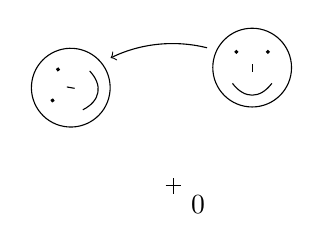
\begin{tikzpicture}
\draw (0,-.1) -- (0,.1);
\draw (-.1, 0) -- (.1, 0) node[anchor = north west]{0};

\draw (1,1.5) circle (.5cm);
\draw (1,1.45) -- (1,1.55);
\filldraw (.8, 1.7) circle (.5pt);
\filldraw (1.2, 1.7) circle (.5pt);
\draw (.75,1.3) .. controls (.9,1.1) and (1.1,1.1) .. (1.25,1.3);

\begin{scope}[rotate=80]
\draw (1,1.5) circle (.5cm);
\draw (1,1.45) -- (1,1.55);
\filldraw (.8, 1.7) circle (.5pt);
\filldraw (1.2, 1.7) circle (.5pt);
\draw (.75,1.3) .. controls (.9,1.1) and (1.1,1.1) .. (1.25,1.3);
\end{scope}
\draw[->, rotate=20] (1,1.5) arc (56:96:1.8);
\end{tikzpicture}
\quad
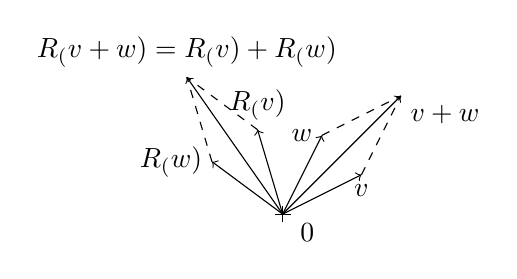
\begin{tikzpicture}
\draw (0,-.1) -- (0,.1);
\draw (-.1, 0) -- (.1, 0) node[anchor = north west]{0};

\draw[->] (0,0) -- (1,.5) node[anchor = north]{$v$};
\draw[->] (0,0) -- (.5,1) node[anchor = east]{$w$};
\draw[dashed] (1,.5) -- (1.5,1.5);
\draw[dashed] (.5,1) -- (1.5,1.5);
\draw[->] (0,0) -- (1.5,1.5) node[anchor = north west]{$v+w$};

\begin{scope}[rotate = 80]
\draw[->] (0,0) -- (1,.5) node[anchor = south]{$R_\ph(v)$};
\draw[->] (0,0) -- (.5,1) node[anchor = east]{$R_\ph(w)$};
\draw[dashed] (1,.5) -- (1.5,1.5);
\draw[dashed] (.5,1) -- (1.5,1.5);
\draw[->] (0,0) -- (1.5,1.5) node[anchor = south]{$R_\ph(v+w)=R_\ph(v)+R_\ph(w)$};
\end{scope}
\end{tikzpicture}
\quad
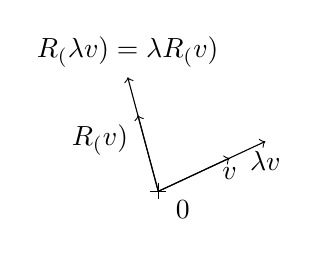
\begin{tikzpicture}
\draw (0,-.1) -- (0,.1);
\draw (-.1, 0) -- (.1, 0) node[anchor = north west]{0};

\draw[->] (0,0) -- +(25:1) node[anchor = north]{$v$};
\draw[->] (0,0) -- +(25:1.5) node[anchor = north]{$\lambda v$};

\begin{scope}[rotate = 80]
\draw[->] (0,0) -- +(25:1) node[anchor = north east]{$R_\ph(v)$};
\draw[->] (0,0) -- +(25:1.5) node[anchor = south]{$R_\ph(\lambda v)=\lambda R_\ph(v)$};
\end{scope}
\end{tikzpicture}
\end{center}
\item $S:\R^2\to \R^2,\cvec{x\\y}\mapsto \cvec{-x\\y}$ Spiegelung an der zweiten Koordinatenachse.
\begin{center}
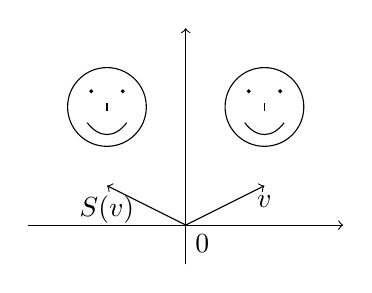
\begin{tikzpicture}
\draw (0, 0) node[anchor = north west]{0};
\draw[->] (-2,0) -- (2,0);
\draw[->] (0,-.5) -- (0,2.5);

\draw (1,1.5) circle (.5cm);
\draw (1,1.45) -- (1,1.55);
\filldraw (.8, 1.7) circle (.5pt);
\filldraw (1.2, 1.7) circle (.5pt);
\draw (.75,1.3) .. controls (.9,1.1) and (1.1,1.1) .. (1.25,1.3);

\draw[->] (0,0) -- (1,.5) node[anchor = north]{$v$};

\draw (-1,1.5) circle (.5cm);
\draw (-1,1.45) -- (-1,1.55);
\filldraw (-.8, 1.7) circle (.5pt);
\filldraw (-1.2, 1.7) circle (.5pt);
\draw (-.75,1.3) .. controls (-.9,1.1) and (-1.1,1.1) .. (-1.25,1.3);

\draw[->] (0,0) -- (-1,.5) node[anchor = north]{$S(v)$};
\end{tikzpicture}
\end{center}
\item $P:\R^2\to \R^2,\cvec{x\\y}\mapsto\cvec{x\\0}$ Projektion auf die erste Koordinatenachse.
\begin{center}
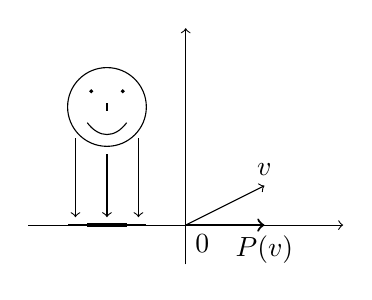
\begin{tikzpicture}
\draw (0, 0) node[anchor = north west]{0};
\draw[->] (-2,0) -- (2,0);
\draw[->] (0,-.5) -- (0,2.5);

\draw (-1,1.5) circle (.5cm);
\draw (-1,1.45) -- (-1,1.55);
\filldraw (-.8, 1.7) circle (.5pt);
\filldraw (-1.2, 1.7) circle (.5pt);
\draw (-.75,1.3) .. controls (-.9,1.1) and (-1.1,1.1) .. (-1.25,1.3);

\draw[->] (0,0) -- (1,.5) node[anchor = south]{$v$};

\draw[->, thick] (0,0) -- (1,0) node[anchor = north]{$P(v)$};

\draw[thick] (-.5,0) -- (-1.5,0);
\draw[very thick] (-1,0) -- (-1,0);
\draw[very thick] (-.75,0) -- (-1.25,0);

\draw[->] (-1, .9) -- (-1,.1);
\draw[->] (-1.4,1.1) -- (-1.4,.1);
\draw[->] (-.6,1.1) -- (-.6,.1);
\end{tikzpicture}
\end{center}
\item $T_a:\R^2\to \R^2, \cvec{x\\y}\mapsto\cvec{x+ay\\y}$ Scherung an der ersten Koordinatenachse um $a\in\R$.
\begin{center}
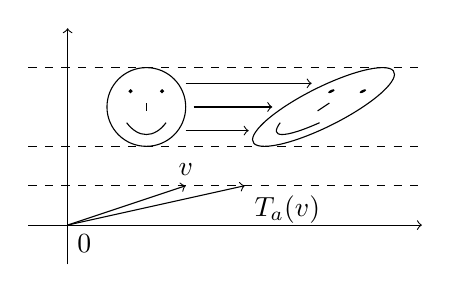
\begin{tikzpicture}
\draw (0, 0) node[anchor = north west]{0};
\draw[->] (-.5,0) -- (4.5,0);
\draw[->] (0,-.5) -- (0,2.5);

\draw[->] (0,0) -- (1.5,.5) node[anchor = south]{$v$};
\draw[dashed] (-.5,.5) -- (4.5,.5);
\draw[dashed] (-.5,2) -- (4.5,2);
\draw[dashed] (-.5,1) -- (4.5,1);

\draw (1,1.5) circle (.5cm);
\draw (1,1.45) -- (1,1.55);
\filldraw (.8, 1.7) circle (.5pt);
\filldraw (1.2, 1.7) circle (.5pt);
\draw (.75,1.3) .. controls (.9,1.1) and (1.1,1.1) .. (1.25,1.3);

\begin{scope}[xslant = 1.5]
\draw (1,1.5) circle (.5cm);
\draw (1,1.45) -- (1,1.55);
\filldraw (.8, 1.7) circle (.5pt);
\filldraw (1.2, 1.7) circle (.5pt);
\draw (.75,1.3) .. controls (.9,1.1) and (1.1,1.1) .. (1.25,1.3);

\draw[->] (0,0) -- (1.5,.5) node[anchor = north west]{$T_a(v)$};
\end{scope}

\draw[->] (1.6, 1.5) -- (2.6,1.5);
\draw[->] (1.5, 1.8) -- (3.1,1.8);
\draw[->] (1.5, 1.2) -- (2.3,1.2);
\end{tikzpicture}
\end{center}
\item Sei $A\in K^{m\times n}$. Dann ist $f_A: K^n\to K^m, x\mapsto Ax$ [$\to$ \ref{5.1.9}] linear (nachrechnen!). Es gilt $\ker f_A = \ker A$ [$\to$ \ref{2.3.10}(b), \ref{5.3.1}]. Weiter ist $\im A :=\im f_A$ [$\to$ \ref{2.3.13}] der von den Spalten von $A$ aufgespannte Unterraum von $K^m$, den wir auch den \emph{Spaltenraum}\index{Matrix@{\bf Matrix}!Spaltenraum} von $A$ (vgl. auch \ref{5.3.1}) oder das \emph{Bild}\index{Matrix@{\bf Matrix}!Bild} von $A$ nennen.
\item $D:K[X]\to K[X], \sum_{k=0}^{n}a_kX^k\mapsto\sum_{k=1}^{n}k a_k X^{k-1}$ $(n\in \N_0, a_0,\ldots,a_n\in K)$ mit $k=\underbrace{1+\ldots+1}_{k\text{-mal}}\in K$.\\
$D^{(d)}:K[X]_d\to K[X]_d, p\mapsto Dp$ $[d\in \N_0]$ formale Ableitung.
\item $E_{a_1,\ldots,a_n}: K[X]\to K^n, p\mapsto \cvec{p(a_1)\\\vdots\\p(a_n)}$ $[n\in\N_0, a_1,\ldots,a_n\in K]$.\\
$E_{a_1,\ldots,a_n}^{(d)}:K[X]_d\to K^n, p\mapsto\cvec{p(a_1)\\\vdots\\p(a_n)}$ $[d\in\N_0]$
\item Die komplexe Konjugation $C:\C\to \C, z\mapsto z^*$ ist $\R$-linear, aber nicht $\C$-linear. In der Tat: $C$ ist nach \ref{4.2.7} ein Automorphismus des kommutativen Ringes $\C$, insbesondere der additiven Gruppe von $\C$. Es gilt $C(\lambda z)=(\lambda z)^* = \lambda^*z^* =\lambda z^* = \lambda C(z)$ für alle $\lambda\in \R$ und $z\in \C$, aber $C(\i 1)=-\i\ne \i = \i C(1)$.
\end{enumerate}
\end{bsp}

\begin{pro}\label{6.3.3}
Seien $U,V,W$ $K$-Vektorräume.
\begin{enumerate}[\rm(a)]
\item Sind $U\xrightarrow{f}V\xrightarrow{g}W$ Vektorraumhomomorphismen, so auch $g\circ f$.
\item Ist $f:V\to W$ ein Vektorraumisomorphismus, so auch $f^{-1}$.
\end{enumerate}
\end{pro}
\begin{proof}
Nach \ref{2.2.14} muss jeweils nur noch die Homogenität [$\to$ \ref{6.3.1}] nachgerechnet werden.
\begin{enumerate}[\normalfont(a)]
\item Sind $U\xrightarrow{f} V\xrightarrow{g} W$ Vektorraumhomomorphismen, $u\in U$ und $\lambda\in K$, so
$$(g\circ f)(\lambda u) = g(f(\lambda u)) = g(\lambda f(u)) = \lambda g(f(u)) = \lambda(g\circ f)(u).$$
\item Sind $f:V\to W$ ein Vektorraumisomorphismus, $w\in W$ und $\lambda\in K$, so
\begin{align*}
f(f^{-1}(\lambda w)) & = (f\circ f^{-1})(\lambda w) = \id_W(\lambda w) = \lambda w = \lambda \id_W(w) = \lambda(f\circ f^{-1})(w)\\
& = \lambda (f(f^{-1}(w))) \overset{f\text{ Hom.}}{=} f(\lambda f^{-1}(w))
\end{align*}
und daher $f^{-1}(\lambda w) = \lambda f^{-1}(w)$, da $f$ injektiv ist.
\end{enumerate}
\end{proof}

\begin{pro}\label{6.3.4}
Seien $V$ und $W$ $K$-Vektorräume, $B\subseteq V$ und $g:B\to W$. Ist $B$\\
\case{eine Basis}{ein Erzeugendensystem} von $V$, so gibt es \case{genau}{höchstens} eine lineare Abbildung $f:V\to W$ mit $f|_B = g$.
\end{pro}
\begin{proof}
Seien zunächst $B$ ein Erzeugendensystem von $V$ und $f_1,f_2:V\to W$ linear mit $f_1|_B = g = f_2|_B$. Zu zeigen: $f_1=f_2$. Sei $v\in V$. Wegen $V=\lin B$ gibt es $n\in\N_0, v_1,\ldots,v_n\in B$ und $\lambda_1,\ldots,\lambda_n\in B$ mit $v=\sum_{i=1}^{n}\lambda_iv_i$. Dann gilt
$$f_1(v) = \sum_{i=1}^{n}\lambda_i f_1(v_i) = \sum_{i=1}^{n}\lambda_ig(v_i) = \sum_{i=1}^{n}\lambda_i f_2(v_i) = f_2(v).$$
Sei nun $B$ sogar eine Basis von $V$. Dann gibt es für jedes $v\in V$ eine eindeutig bestimmte Familie $(\lambda_u)_{u\in B}$ in $K$ mit endlichem Träger $\left\{u\in B\mid \lambda_u\ne 0\right\}$ und $v=\sum_{u\in B} \lambda_u u :=\sum_{\substack{u\in B\\\lambda_u\ne 0}}\lambda_u u$. Daher ist
$$f:V\to W, \sum_{u\in B}\lambda_u u\mapsto\sum_{u\in B}\lambda_u g(u)\qquad ((\lambda_u)_{u\in B}\in K^B \text{ mit endlichem Träger})$$
eine wohldefinierte Abbildung.
Zu zeigen: $f$ linear. Seien $(\lambda_u)_{u\in B}$ und $(\mu_u)_{u\in B}$ Familien in $K$ mit endlichen Trägern und $\lambda\in K$.\\
Dann 
\begin{align*}
f\left(\sum_{u\in B}\lambda_u u+\sum_{u\in B}\mu_u u\right) & \overset{\text{\ref{6.1.1} (D')}}{=} f\left(\sum_{u\in B}(\lambda_u+\mu_u)u\right)\\
& = \sum_{u\in B}(\lambda_u +\mu_u)g(u) \overset{\text{(D')}}{=} \sum_{u\in B}\lambda_u g(u) + \sum_{u\in B}\mu_u g(u)\\
& = f\left(\sum_{u\in B}\lambda_u u\right) + f\left(\sum_{u\in B}\mu_u u\right) \quad \text{und}
\end{align*}
\begin{align*}
f\left(\lambda\sum_{u\in B}\lambda_u u\right) & \overset{\text{\vecD}}{=} f\left(\sum_{u\in B}\lambda(\lambda_u u)\right) \overset{\text{(V)}}{=} f\left(\sum_{u\in B}(\lambda\lambda_u) u\right) = \sum_{u\in B}(\lambda\lambda_u)g(u)\\
& \overset{\text{(V)}}{=}\sum_{u\in B}\lambda(\lambda_u g(u)) \overset{\text{\vecD}}{=}\lambda\sum_{u\in B}\lambda_u g(u)=\lambda f\left(\sum_{u\in B}\lambda_u u\right).
\end{align*}
\end{proof}

\begin{bsp}\label{6.3.5}
\begin{enumerate}[\normalfont(a)]
\item Um zu zeigen, dass für alle $p\in \R[X]_2$ gilt:
$$(*)\qquad \int_{-1}^{1}p(x)\,dx =  p\left(\frac{1}{\sqrt{3}}\right)+p\left(-\frac{1}{\sqrt{3}}\right),$$
reicht es wegen der Linearität der beiden Abbildungen $\R[X]_2\to \R, p\mapsto\int_{-1}^{1}p(x)\,dx$ und $\R[X]_2\to \R, p\mapsto p\left(\frac{1}{\sqrt{3}}\right)+p\left(-\frac{1}{\sqrt{3}}\right)$ zu zeigen, dass $(*)$ für alle $p\in \left\{1,X,X^2\right\}$ gilt, denn $\left\{1,X,X^2\right\}$ erzeugt den $\R$-Vektorraum $\R[X]_2$.
$$\int_{-1}^{1}1\, dx = 2 = 1+1$$
$$\int_{-1}^{1}x\, dx = 0 = \frac{1}{\sqrt{3}}-\frac{1}{\sqrt{3}}$$
$$\int_{-1}^{1}x^2\, dx = \left[\frac{x^3}{3}\right]_{x = -1}^{1}= \frac{1}{3}+\frac{1}{3} = \left(\frac{1}{\sqrt{3}}\right)^2 +\left(-\frac{1}{\sqrt{3}}\right)^2$$
\item Die formale Ableitung $D:K[X]\to K[X]$ aus \ref{6.3.2} (f) hätte man wegen \ref{6.2.8}(d) auch wie folgt definieren können: "`Sei $D\colon K[X]\to K[X], 1\mapsto 0 , X^k\mapsto kX^{k-1}$ $(k\in \N)$ linear."'
\end{enumerate}
\end{bsp}

\begin{pro}\label{6.3.6}
Seien $V$ ein $K$-Vektorraum, $v_1,\ldots,v_n\in V$ und $\underline{v}=(v_1,\ldots,v_n)$. Die Abbildung $\ve_{\underline{v}}: K^n \to V, \cvec{\lambda_1\\\vdots\\\lambda_n}\mapsto \sum_{i=1}^{n}\lambda_i v_i$ ist linear. Sie ist \caset{injektiv}{bijektiv}{surjektiv} genau dann, wenn $v_1,\ldots,v_n$ \caset{linear unabhängig in $V$ sind}{eine Basis von $V$ bilden}{$V$ erzeugen}.
\end{pro}
\begin{proof}
Man rechnet sofort nach, dass $\ve_{\underline{v}}$ linear ist (diese Rechnung sahen wir allgemeiner schon im Beweis von
Proposition \ref{6.3.4}, denn $\ve_{\underline{v}}$ ist
die eindeutig bestimmte lineare Abbildung $K^n\to V$ ist, die $e_i$ [$\to$ \ref{6.2.2}] auf $v_i$ abbildet).
Es gilt
\begin{align*}
\ve_{\underline{v}}\text{ injektiv}&\iff\ker\ve_{\underline{v}} = \left\{0\right\}\overset{\text{\ref{6.2.3}(a)}}{\iff}
v_1,\ldots,v_n\text{ linear unabhängig in }V\qquad\text{und}\\
\ve_{\underline{v}}\text{ surjektiv}&\iff\im\ve_{\underline{v}}=V\overset{\text{\ref{6.2.1}(a)}}{\iff} v_1,\ldots,v_n
\text{ erzeugen }V.
\end{align*}
\end{proof}

\begin{notpro}\label{6.3.7}
Sei $\underline{v}=(v_1,\ldots,v_n)$ eine Basis des $K$-Vektorraums $V$. Dann sind
$$\ve_{\underline{v}}:K^n\to V,\cvec{\lambda_1\\\vdots\\\lambda_n}\mapsto \sum_{i=1}^{n}\lambda_iv_i \quad \text{und}$$
$$\co_{\underline{v}}:=\ve_{\underline{v}}^{-1}:V\to K^n,\sum_{i=1}^{n}\lambda_iv_i\mapsto\underbrace{\cvec{\lambda_1\\\vdots\\\lambda_n}}_\text{"`Koordinaten"'}\quad(\lambda_1,\ldots,\lambda_n\in K)$$
nach \ref{6.3.6} und \ref{6.3.3} Vektorraumisomorphismen.\index{Vektorraum@{\bf Vektorraum}!Homomorphismus/ lineare Abbildung!co@$\co_\v$}\index{Vektorraum@{\bf Vektorraum}!Homomorphismus/ lineare Abbildung!ve@$\ve_\v$}
\end{notpro}

\begin{sat}\label{6.3.8}
Sei $V$ ein $K$-Vektorraum mit Basis $\underline{v}= (v_1,\ldots,v_n)$. Sei $W$ ein weiterer $K$-Vektorraum und $f:V\to W$ linear. Genau dann ist $f$ \caset{injektiv}{bijektiv}{surjektiv}, wenn $f(v_1),\ldots,f(v_n)$ \caset{linear unabhängig in $W$ sind}{eine Basis von $W$ bilden}{$W$ erzeugen}.
\end{sat}
\begin{proof}
$K^n\xrightarrow{\ve_{\underline{v}}}V\xrightarrow{f}W$\\
Da $\ve_{\underline{v}}$ bijektiv ist, kann man $f$ durch $f\circ \ve_{\underline{v}}$, $V$ durch $K^n$ und $\v$ durch $\e$ ersetzen. Wende nun \ref{6.3.6} an unter Beachtung von $f\circ \ve_\v = \ve_{(f(v_1),\ldots,f(v_n))}$.
\end{proof}

\begin{df}\mbox{}\label{6.3.9}
[$\to$ \ref{2.2.15}] Zwei $K$-Vektorräume $V$ und $W$ heißen \emph{isomorph}\index{Vektorraum@{\bf Vektorraum}!isomorph ($\cong$)}, wenn es einen Isomorphismus von $V$ nach $W$ gibt, in Zeichen $V\cong W$.
\end{df}

\begin{sat}\label{6.3.10}
Seien $V$ und $W$ $K$-Vektorräume, von denen mindestens einer endlichdimensional ist. Dann $V\cong W\iff \dim V = \dim W$.
\end{sat}
\begin{proof}
\OE ~ $V$ endlichdimensional [$\to$ \ref{6.2.25}(d)], etwa mit Basis $(v_1,\ldots,v_n)$ [$\to$ \ref{6.2.22}].
\begin{itemize}
\item["`$\Longrightarrow$"'] Gelte $V\cong W$. Wähle Isomorphismus $f:V\to W$. Dann $(f(v_1),\ldots,f(v_n))$ Basis von $W$ [$\to$ \ref{6.3.8}]. Also $\dim V=\dim W$ [$\to$ \ref{6.2.24}].
\item["`$\Longleftarrow$"'] Gelte $\dim V= \dim W$. Dann $\dim W=n$, d.h. es gibt eine Basis $(w_1,\ldots,w_n)$ von $W$. Definiere lineare Abbildung $f:V\to W, v_i\mapsto w_i$ [$\to$ \ref{6.3.4}]. Nach \ref{6.3.8} ist $f$ bijektiv, also ein Isomorphismus.
\end{itemize}
\end{proof}

\begin{kor}\label{6.3.11}
Jeder Vektorraum der Dimension $n\in \N_0$ ist isomorph zu $K^n$.
\end{kor}

\begin{bem}\label{6.3.12}
"`Bis auf Isomorphie"' gibt es also keine anderen endlichdimensionalen $K$-Vektorräume als die $K^n$ $(n\in \N_0)$. Dabei entspricht die Wahl einer geordneten Basis [$\to$ \ref{6.2.1}(c)] der Wahl eines Isomorphismus:
\end{bem}

\begin{sat}\label{6.3.13}
Sei $V$ ein $K$-Vektorraum mit $n:=\dim V <\infty$. Die Zuordnungen
\begin{align*}
\underline{v} & \mapsto \ve_{\underline{v}}\\
(f(e_1),\ldots,f(e_n)) & \mapsfrom f
\end{align*}
vermitteln eine Bijektion {\rm[$\to$ \ref{1.2.7}]} zwischen der Menge der geordneten Basen von $V$ und der Menge der Vektorraumisomorphismen $K^n\to V$.
\end{sat}
\begin{proof}
Zu zeigen:
\begin{enumerate}[\normalfont(a)]
\item Ist $\underline{v}$ Basis von $V$, so ist $\ve_{\underline{v}}$ ein Isomorphismus.
\item Ist $f:K^n\to V$ ein Isomorphismus, so $(f(e_1),\ldots,f(e_n))$ Basis von $V$.
\item Ist $\underline{v} = (v_1,\ldots,v_n)$ Basis von $V$, so gilt $\underline{v} = (\ve_{\underline{v}}(e_1),\ldots,\ve_{\underline{v}}(e_n))$.
\item Ist $f:K^n\to V$ ein Isomorphismus, so $f=\ve_{(f(e_1),\ldots,f(e_n))}$.
\end{enumerate}
(a) folgt aus \ref{6.3.6}, (b) aus \ref{6.3.8}, (c) aus \ref{6.3.7} und (d) aus \ref{6.3.4}.
\end{proof}

\red{Bis hierher sollten wir am 20. Dezember kommen.}
\end{document}